\documentclass[11pt]{article}
\pdfpxdimen=1in
\divide\pdfpxdimen by 300
 
\usepackage[latin1]{inputenc}
\usepackage[T1]{fontenc}
\usepackage[english]{babel}
\usepackage{mathtools, bm}
\usepackage{amsmath,amssymb,amsthm}
\usepackage{mathrsfs}
\usepackage{cancel}
\usepackage{float}

\usepackage{caption} % to center captions
\usepackage{subcaption} % subcaption for figures side by side

\usepackage{booktabs} % for super cool table
\usepackage[table,xcdraw]{xcolor}  % to put color in tables
\usepackage{tcolorbox} % add box
\usepackage{commath} % for absolute values
\usepackage{stackengine} % to stack things over equal

\usepackage[parfill]{parskip}
\usepackage{graphicx}
\usepackage{hyperref}
\usepackage[top=0.8in, bottom=0.8in, left=1in, right=1in]{geometry}
\usepackage{listings}
\usepackage{minted}
\usepackage{framed}

% D( p || q)
\DeclarePairedDelimiterX{\infdivx}[2]{(}{)}{%
  #1\;\delimsize\|\;#2%
}
\newcommand{\infdiv}{D\infdivx}

\renewcommand\thesubsection{\thesection.\arabic{subsection}} % Subsection starting with A, B, ...

\renewcommand\thefigure{\thesubsection.\arabic{figure}}

\newcommand{\horrule}[1]{\rule{\linewidth}{#1}} % Create horizontal rule command with 1 argument of height

\numberwithin{figure}{section} % to have per-section figure numbering

% to use independent and not independent signs %
\makeatletter
\newcommand*{\indep}{%
  \mathbin{%
    \mathpalette{\@indep}{}%
  }%
}
\newcommand*{\nindep}{%
  \mathbin{%                   % The final symbol is a binary math operator
    %\mathpalette{\@indep}{\not}% \mathpalette helps for the adaptation
    \mathpalette{\@indep}{/}%
                               % of the symbol to the different math styles.
  }%
}
\newcommand*{\@indep}[2]{%
  % #1: math style
  % #2: empty or \not
  \sbox0{$#1\perp\m@th$}%        box 0 contains \perp symbol
  \sbox2{$#1=$}%                 box 2 for the height of =
  \sbox4{$#1\vcenter{}$}%        box 4 for the height of the math axis
  \rlap{\copy0}%                 first \perp
  \dimen@=\dimexpr\ht2-\ht4-.2pt\relax
      % The equals symbol is centered around the math axis.
      % The following equations are used to calculate the
      % right shift of the second \perp:
      % [1] ht(equals) - ht(math_axis) = line_width + 0.5 gap
      % [2] right_shift(second_perp) = line_width + gap
      % The line width is approximated by the default line width of 0.4pt
  \kern\dimen@
  \ifx\\#2\\%
  \else
    \hbox to \wd2{\hss$#1#2\m@th$\hss}%
    \kern-\wd2 %
  \fi
  \kern\dimen@
  \copy0 %                       second \perp
}
\makeatother

\title{	
\normalfont \normalsize 
\textsc{Master MVA \\
Probabilistic Graphical Models} \\ [20pt]
\horrule{0.5pt} \\[0.2cm] % Thin top horizontal rule
\textbf{Homework 3}: HMM \\
\horrule{2pt} \\[0.3cm] % Thick bottom horizontal rule
}

\author{Victor Busa \\
   \texttt{victor.busa@ens-paris-saclay.fr}}

\date{\normalsize\today}

\begin{document}
\def\useanchorwidth{T}

\maketitle

\section{HMM - Implementation}

\paragraph{1 Recursions $\alpha$ and $\beta$}
To implement $\alpha$, $\beta$ recursions we will use the $log(\sum\limits_{a \in \mathcal{A}} exp(p(a))$ trick. \\
I won't detail the implementation of $\alpha$ and $\beta$
recursion and I will instead focus my attention on the joint probability calculation. The joint probability $\mathbb{P}[q_{t+1} = i, q_t = i | u_0, \hdots, u_T]$ is given by:

\begin{align*}
\mathbb{P}[q_{t+1} = i, q_t = i | u_0, \hdots, u_T] = \dfrac{1}{\mathbb{P}[u_0, \hdots, u_T]} . \alpha_t(q_t) . \beta_{t+1}(q_{t+1}) . \mathbb{P}[q_{t+1} = i, q_t = i]
. \mathbb{P}[u_{t+1} | q_{t+1}=i]
\end{align*}

So, using the logarithm function it comes:

\begin{align*}
log\; \mathbb{P}[q_{t+1} = i, q_t = i | u_0, \hdots, u_T] =& \; \overbrace{-log\;\mathbb{P}[u_0, \hdots, u_T]}^{(1)} + \overbrace{log\; \alpha_t(q_t = j)}^{(2)} + \overbrace{log \;\beta_{t+1}(q_{t+1} = i)}^{(3)} \\
&+\; \underbrace{log \; \mathbb{P}[q_{t+1} = i, q_t = j]}_{(4)}
+ \underbrace{log\; \mathbb{P}[u_{t+1} | q_{t+1}=i]}_{(5)}
\end{align*}

We can rewrite ($1$) as:

\begin{align*}
(1) =& - log\left[\sum\limits_{q_t} \alpha_t(q_t) \beta_t(q_t)\right] \\
=& - \max\limits_{q_t}[log\; \alpha_t(q_t) + log\; \beta_t(q_t)] - log\left[\sum\limits_{q_t} exp\left(log\; \alpha_t(q_t) + log\; \beta_t(q_t) - \max\limits_{q_t}[log\; \alpha_t(q_t) + log\; \beta_t(q_t)]\right)\right]
\end{align*}

In python we can compute such a quantity (1) as follow:

\begin{minted}[linenos=true, tabsize=4, fontfamily=courier, fontsize=\small]{python}
# compute - log(p[uO, ... uT])
pa = (alpha + beta)[0, :]
logsum = np.log(np.sum(np.exp(pa - np.max(pa))))
term1 = np.max(pa) + logsum
			
result -= term1
\end{minted}

terms ($2$, $3$, $4$, $5$) are straightforward to compute as we have:

\begin{align*}
(2) &= log\; \alpha_t(q_t = j) = alpha[t, j] \\
(3) &= log\; \beta_{t+1}(q_{t+1}=i) = beta[t+1, i] \\
(4) &= log\; \mathbb{P}[q_{t+1} = i, q_t = j] = log\; A_{i,j} \\
(5) &= log\; \mathbb{P}[u_{t+1} | q_{t+1}=i] = log\; \mathcal{N}_{t+1}(\mu_i, \Sigma_i)
\end{align*}

As we want the joint probability for all values of $i$, $j$, and $T$ we have to iterates over all these variables, such that the naive
implementation of the joint probability calculation in python can be written as:

\begin{minted}[linenos=true, tabsize=4, fontfamily=courier, fontsize=\small]{python}
def joint_proba(alpha, beta, data, mu, sigma, A):
    (T, K) = alpha.shape
    
    # need to store p[qt+1 = i, qt = j | uo,... uT]
		# for all i, j in {1,...,K} and all t in 0 T-1
    result = np.zeros((T-1, K,K))
    
    # compute - log(p[uO, ... uT])
    pa = (alpha + beta)[0, :]
    logsum = np.log(np.sum(np.exp(pa - np.max(pa))))
    term1 = np.max(pa) + logsum
    
    result -= term1
    
    for t in range(T-1):
        proba_t = np.zeros((K, K))
        
        for i in range(K):
            # proba[i, j] = log(p[qt+1 = i, qt = j | uo,... uT])
            proba_t[i,:] += np.log(multivariate_normal.pdf(data[t+1],
						mean=mu[i], cov=sigma[i])) + beta[t+1, i]
            
            for j in range(K):
                proba_t[i, j] += np.log(A[i,j]) + alpha[t, j]
        
        result[t, :] += proba_t
        
    return np.exp(result)
\end{minted}

\textbf{Note}: The above code is a naive implementation and it is here for explanation reason only. For efficiency sackness the code has been improved by using matrix operation to avoid looping over $i$ and $j$.

\paragraph{2. Smoothing computation}
To compute the smoothing quantity: $p(q_t | u_1, \hdots, u_T)$ we will use the $log(\sum\limits_{a \in \mathcal{A}} exp(p(a))$ trick. Let's
recall that the smoothing quantity is defined as:

\begin{align*}
p(q_t | u_1, \hdots, u_T) &= \frac{\alpha_t(q_t)\beta_t(q_t)}{\sum\limits_{q_t} \alpha_t(q_t) \beta_t(q_t)}
\end{align*}

Thus we have:

\begin{align*}
log \; p(q_t | u_1, \hdots, u_T) &= log \; \alpha_t(q_t) + log \; \beta_t(q_t) - log\left( \sum\limits_{q_t} \alpha_t(q_t) \beta_t(q_t) \right) \\
=&\; log \; \alpha_t(q_t) + log \; \beta_t(q_t) - log\left( \sum\limits_{q_t} exp[log(\alpha_t(q_t) \beta_t(q_t))]\right) \\
=&\; log \; \alpha_t(q_t) + log \; \beta_t(q_t) \; \\
&- log\left( exp\left[\max\limits_{q_t}(log \; \alpha_t(q_t) \beta_t(q_t) )\right] \sum\limits_{q_t} exp \left[log \left(\alpha_t(q_t) \beta_t(q_t) - \max\limits_{q_t}\left(\alpha_t(q_t) \beta_t(q_t)\right)\right) \right]\right) \\
=&\; log \; \alpha_t(q_t) + log \; \beta_t(q_t) \; \\
&- \Bigg( \max\limits_{q_t}(log \; \alpha_t(q_t) + log \; \beta_t(q_t)) \\
&+\; log\left( \sum\limits_{q_t} exp\left[log \left(\alpha_t(q_t) \beta_t(q_t) - \max\limits_{q_t} \left(\alpha_t(q_t) \beta_t(q_t)\right)\right)\right]\right)\Bigg)
\end{align*}

The function \texttt{smoothing(alpha, beta)} exactly use the above identity.

\paragraph{3. Derivation of the estimation equations of the EM algorithm}

As we are dealing with an HMM the complete log-likelihood is (where $\theta = (\pi, A, \{\mu_k, \Sigma_k : k=1,\hdots,4\})$)

\begin{align*}
\ell_c(\theta) &= log \left( p(q_0) \prod\limits_{t=0}^{T-1} p(q_{t+1}|q_t) \prod\limits_{t=0}^T p(u_t | q_t) \right) \\
=& log(p(q_0)) + \sum\limits_{t=0}^{T-1} log \; p(q_{t+1} | q_t) + \sum\limits_{t=0}^T log \; p(u_t | q_t) \\
=& \sum\limits_{i=1}^K \delta(q_0 = i) log \; \pi_i + \sum\limits_{t=0}^{T-1} \sum\limits_{i,j}^K \delta(q_{t+1} = i, q_t = j) log(A_{i,j}) \; \\
&+ \sum\limits_{t=0}^T \sum\limits_{i=1}^K \delta(q_t = i) log\left(\mathcal{N}(u_i, \Sigma_i)\right) \\
=& \sum\limits_{i = 1}^K \delta(q_0 =i) log \; \pi_i + \sum\limits_{t=0}^{T-1} \sum\limits_{i,j}^K \delta(q_{t+1} = i, q_t = j) log(A_{i,j}) \; \\
& -\frac{1}{2} \sum\limits_{t=0}^T \sum\limits_{i=1}^K \delta(q_t = i)\left( log |\Sigma_i| + (u_t - \mu_i)^T \Sigma^{-1}_i (u_t - \mu_i)\right)
- \frac{T.K.d}{2} log \; 2\pi
\end{align*}

\textbf{E-Step}: We want to compute the quantity $\mathbb{E}_{q|u}[\ell_c(\theta)]$ but as we have:

\begin{align}
\mathbb{E}_{q|u}[\delta(q_o = i)] &= \mathbb{P}[q_0 = i | u; \theta^{k-1}] \\
\mathbb{E}_{q|u}[\delta(q_{t+1} = i, q_t = j)] &= \mathbb{P}[q_{t+1} = i, q_t = i | u; \theta^{k-1}] \\
\mathbb{E}_{q|u}[\delta(q_t = i)] &= \mathbb{P}[q_t = i | u; \theta^{k-1}]
\end{align}

it comes:

\begin{align*}
\mathbb{E}_{q|u}[\ell_c(\theta)] =& \sum\limits_{i=1}^K \mathbb{P}[q_0 = i | u; \theta^{k-1}] log \; \pi_i + \sum\limits_{t=0}^{T-1} \sum\limits_{i,j}^K \mathbb{P}[q_{i+1} = i, q_t = i | u; \theta^{k-1}] log \; A_{i,j} \\
&-\frac{1}{2} \sum\limits_{t=0}^T \sum\limits_{i=1}^K \mathbb{P}[q_t = i | u; \theta^{k-1}] \left(log|\Sigma_i| + (u_t -\mu_i)^T \Sigma^{-1}_i (u_t - \mu_i)\right) + cst
\end{align*}

\textbf{M-Step}: We want to maximize w.r.t each parameter. Recall that here $\theta = (\pi, A, \{\mu_k, \Sigma_k : k=1,\hdots,4\})$ \\
$\pi_k$: $f: \pi_i \rightarrow \sum\limits_{i=1}^K \mathbb{P}[q_0 = i | u; \theta^{k-1}] log \; \pi_i$ is strictly concave as a positive weighted sum of logarithm functions which are
strictly concave on their domain. So we can recover the minimum by annulling the gradient of f w.r.t $\pi_i$. Using the condition $\sum\limits_{i=1}^K \pi_i = 1$ we can write the Lagrangian as:

\begin{align*}
\mathcal{L}(\pi, \lambda) = \sum\limits_{i=1}^K \mathbb{P}[q_0 = i | u; \theta^{k-1}] log \; \pi_i + \lambda \left(1 - \sum\limits_{i=1}^K \pi_i\right)
\end{align*}

from what follows:

\begin{align*}
\frac{\partial \mathcal{L}(\pi_i, \lambda)}{\partial \pi_i} = 0 \\
\Leftrightarrow \frac{\mathbb{P}[q_0 = i | u; \theta^{k-1}]}{\pi_i} - \lambda = 0 \\
\Leftrightarrow \lambda \pi_i = \mathbb{P}[q_0 = i | u; \theta^{k-1}]
\end{align*}

Then using the condition $\sum\limits_{i=1}^K \pi_i = 1$, it comes:

\begin{align*}
\lambda \underbrace{\sum\limits_{i=1}^K \pi_i}_{=1} = \sum\limits_{i=1}^K \mathbb{P}[q_0 = i | u; \theta^{k-1}] \triangleq 1
\end{align*}

So finally:

\begin{framed}
\begin{align*}
\pi^k_i = \mathbb{P}[q_0 = i | u; \theta^{k-1}]
\end{align*}
\end{framed}

where $\pi^k_i$ means the $i^{th}$ component of $\pi$ at time $k$. \\
\\

$A$: We want to maximize $g : A_{i,j} \rightarrow \sum\limits_{t=0}^{T-1} \sum\limits_{i,j}^K \mathbb{P}[q_{t+1} = j, q_t = i | u; \theta^{k-1}] log \; A_{i,j}$ w.r.t $A_{i,j}$. g
is a strictly concave function as a positive weighted sum of logarithm functions strictly concave on their domain. Using the condition: $\sum\limits_{j=1}^K A_{i,j} = 1$ (Warning: 
$\sum\limits_{i} A_{i,j} \neq 1$ !!) we can write the Lagrangian as:

\begin{align*}
\mathcal{L}(A_{i,j}, \lambda) = \sum\limits_{t=0}^{T-1} \sum\limits_{i,j = 1}^K \mathbb{P}[q_{t+1} = j, q_t = i | u; \theta^{k-1}] log \; A_{i,j} + \lambda(1 - \sum\limits_{j=1}^K A_{i,j})
\end{align*}

We can recover the minimum by annulling the gradient of g as g is a strictly concave function on its domain:

\begin{align*}
\frac{\partial \mathcal{L}(A_{i,j}, \lambda)}{\partial A_{i,j}} = \frac{\sum\limits_{t=0}^{T-1} \mathbb{P}[q_{t+1} = j, q_t = i | u; \theta^{k-1}]}{A_{i,j}} - \lambda = 0
\end{align*}

Then, using the condition $\sum\limits_{j=1}^K A_{i,j} = 1$ it comes:

\begin{align*}
\lambda \underbrace{\sum\limits_{j=1}^K A_{i,j}}_{= 1} = \sum\limits_{t=0}^{T-1} \sum\limits_{j=1}^K  \mathbb{P}[q_{t+1} = j, q_t = i | u; \theta^{k-1}]
\end{align*}

So finally:
\begin{framed}
\begin{align*}
A_{i,j}^k = \frac{\sum\limits_{t=0}^{T-1} \mathbb{P}[q_{t+1} = j, q_t = i | u; \theta^{k-1}]}{\lambda} = \frac{\sum\limits_{t=0}^{T-1} \mathbb{P}[q_{t+1} = j, q_t = i | u; \theta^{k-1}]}{\sum\limits_{t=0}^{T-1} \sum\limits_{j'=1}^K  \mathbb{P}[q_{t+1} = j', q_t = i | u; \theta^{k-1}]}
\end{align*}
\end{framed}

Where $A_{i,j}^k$ refers to the value of $A_{i,k}$ at time $k$. \\
\\

$mu_k$: We want to maximize $h : \mu_k \rightarrow -\frac{1}{2} \sum\limits_{t=0}^{T} \sum\limits_{i=1}^K \mathbb{P}[q_t = i | u; \theta^{k-1}] (u_t - \mu_i)^T \Sigma^{-1}_i (u_t - \mu_i)$ w.r.t $\mu_k$,, $\forall k \in \{1,2,3,4\}$. h is a concave function as it is the sum of the opposite of quadratic forms ($\Sigma_i$ positive semi-definite and so do $\Sigma^{-1}$), so we can recover the maximum of $h$ by annulling the gradient of $h$:

\begin{align*}
-\frac{1}{2} \nabla_{\mu_i} \left( \sum\limits_{t=0}^{T} \sum\limits_{i=1}^K \mathbb{P}[q_t = i | u; \theta^{k-1}] (u_t - \mu_i)^T \Sigma^{-1}_i (u_t - \mu_i) \right) = 0 \\
\Leftrightarrow \Sigma^{-1}_i \sum\limits_{t=0}^T \mathbb{P}[q_t = i | u; \theta^{k-1}] (u_t - \mu_i) = 0 \\
\Leftrightarrow \mu_i = \frac{\sum\limits_{t=0}^T \mathbb{P}[q_t = i | u; \theta^{k-1}] u_t}{\sum\limits_{t=0}^T \mathbb{P}[q_t = i | u; \theta^{k-1}]}
\end{align*}

where we have used the fact that $\Sigma^{-1}_i$ is invertible $\forall i \in \{1,2,3,4\}$ in the last equivalence.

Hence, finally we have, $\forall i \in \{1,2,3,4\}$:
\begin{framed}
\begin{align*}
\mu^k_i = \frac{\sum\limits_{t=0}^T \mathbb{P}[q_t = i | u; \theta^{k-1}] u_t}{\sum\limits_{t=0}^T \mathbb{P}[q_t = i | u; \theta^{k-1}]}
\end{align*}
\end{framed}
Where $\mu^k_i$ stands for the $i^{th}$ means at time $k$. \\
\\

$\Sigma_k$: We have already seen this calculation several times in class and in the 2 previous homework, I won't detail the calculation anymore here as it is a bit cubersome. At the end we have:

\begin{framed}
\begin{align*}
\Sigma^k_i = \frac{\sum\limits_{t=0}^T \mathbb{P}[q_t = i | u; \theta^{k-1}] (u_t - \mu^k_i) (u_t - \mu^k_i)^T}{\sum\limits_{t=0}^T \mathbb{P}[q_t = i | u; \theta^{k-1}]}
\end{align*}
\end{framed}

\paragraph{4. Expectation Maximization Implementation} See python code

\paragraph{5. log-likelihood plots}
Using the parameter values computed by the EM algorithm of homework 2, we get the following plots for the log-likelihood:

\begin{figure}[H]
\centering
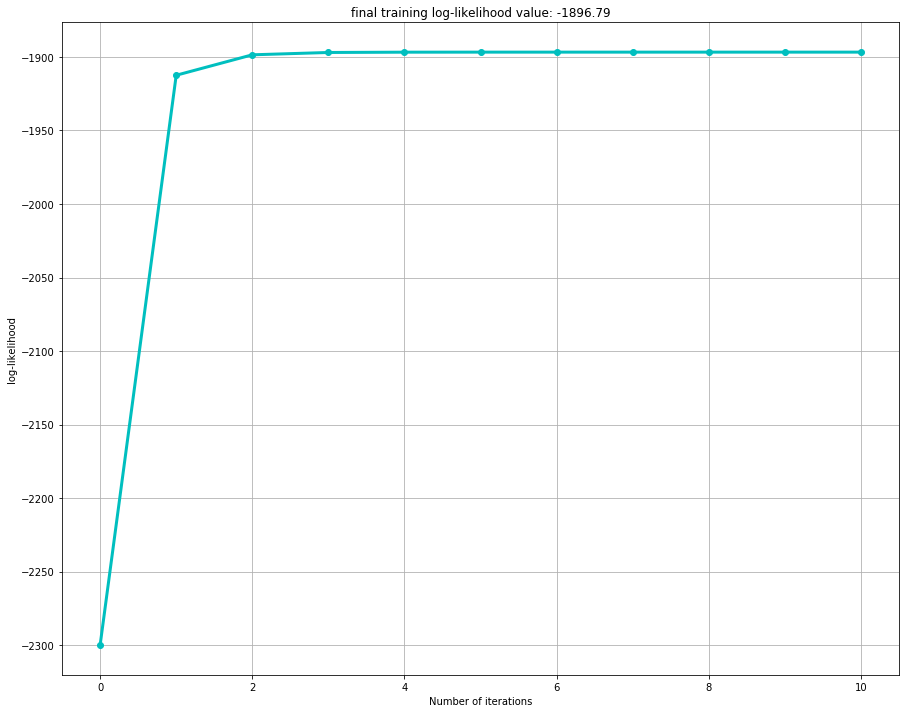
\includegraphics[width=0.75\linewidth]{images/q6_train}
\caption{Log-likelihood plot on the training dataset using the Expectation Maximization algorithm on the HMM}
\label{fig:log_train}
\end{figure}

\begin{figure}[H]
\centering
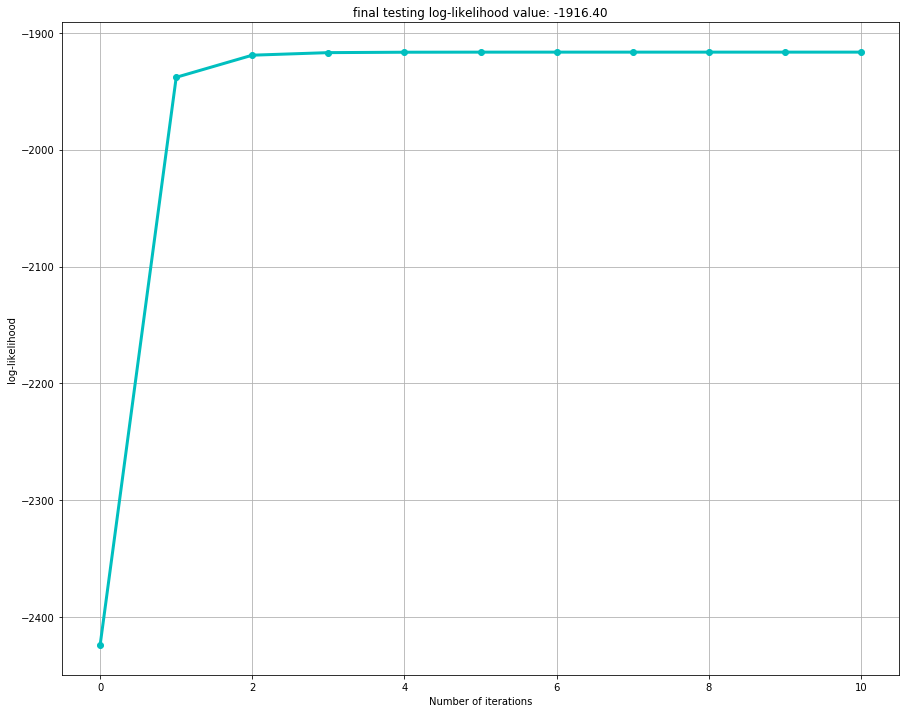
\includegraphics[width=0.75\linewidth]{images/q6_test}
\caption{Log-likelihood plot on the testing dataset using the Expectation Maximization algorithm on the HMM}
\label{fig:log_test}
\end{figure}

\paragraph{6. Comparison of the log-likelihoods}
The Table ~\ref{table:log_comparison} show the different log-likelihood values we obtained using either a Gaussian Mixture Model or an HMM model.

\begin{table}[H]
\centering
\begin{tabular}{|c|c|c|}
\hline
 & \textbf{Gaussian mixture model} & \textbf{Hidden Markov model} \\ \hline
Training set & -2327.72 & -1896.79 \\ \hline
Testing set & -2408.97 & -1916.40 \\ \hline
\end{tabular}
\caption{Log-likehood obtained using either a Gaussian Mixture Model or an HMM}
\label{table:log_comparison}
\end{table}

HMM outperforms the Gaussian Mixture Model because it works on a larger set. It is not a surprise that the log-likelihood is better with the HMM as the GMM can be seen as an HMM without the edges $y_t \rightarrow y_{t+1}$. In other words, HMM should perform better than GMM as it accounts for the same distribution + another set of transitions coming from $y_t \rightarrow y_{t+1}$. It makes sense to compare these models as both of them are Graphical models.

\paragraph{7. Viterbi algorithm}
The Viterbi algorithm estimates the most likely sequence of states, i.e $arg \max_{q_t} \mathbb{P}[q_1, \hdots, q_T | y_1, \hdots, u_T]$. It is the analog
of filtering. It browses the sequence forward, calculating the message $m$ at each step using the same equation as the one for the $\alpha$ recursion were
we have replaced the summation by a maximization. Hence the Viterbi algorithm can be directly derive from the identity:

\begin{align*}
\max\limits_{q_1,..., q_t} \mathbb{P}[q_1, \hdots, q_t, q_{t+1} | u_1, \hdots, u_{t+1}] \\
= \mathbb{P}[u_{t+1} | q_{t+1}] \max_{q_t}\left(\mathbb{P}[q_{t+1} | q_{t}]\max_{q_1, \hdots, q_{t-1}} \mathbb{P}[q_1, \hdots, q_{t-1}, q_t | u_1, \hdots, u_t]\right)
\end{align*}

\paragraph{8. Viterbi decoding}
See code for the implementation of Viterbi algorithm.
The result of applying the Viterbi algorithm to the training dataset in shown on Figure ~\ref{fig:viterbi}

\begin{figure}[H]
\centering
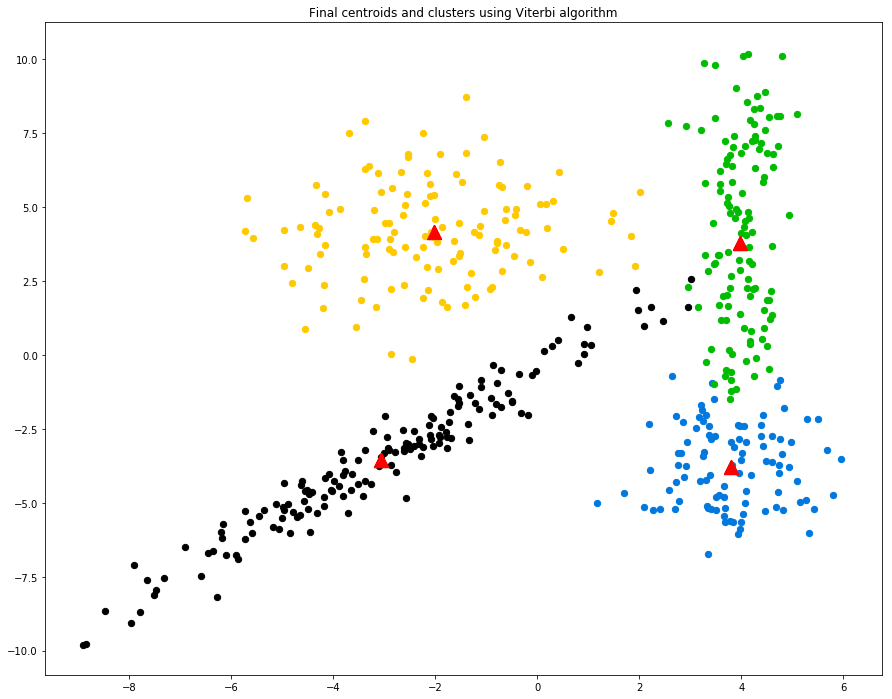
\includegraphics[width=1\linewidth]{images/viterbi}
\caption{Final centroids and clusters using Viterbi algorithm on the training dataset}
\label{fig:viterbi}
\end{figure}

\paragraph{9. Probability plots of $\mathbb{P}[q_t | u_1, \hdots, u_{T}]$ for $T =100$}
The probability plots of $\mathbb{P}[q_t | u_1, \hdots, u_{T}]$ for $T =100$ is shown on Figure~\ref{fig:prob_test}
\begin{figure}[H]
\centering
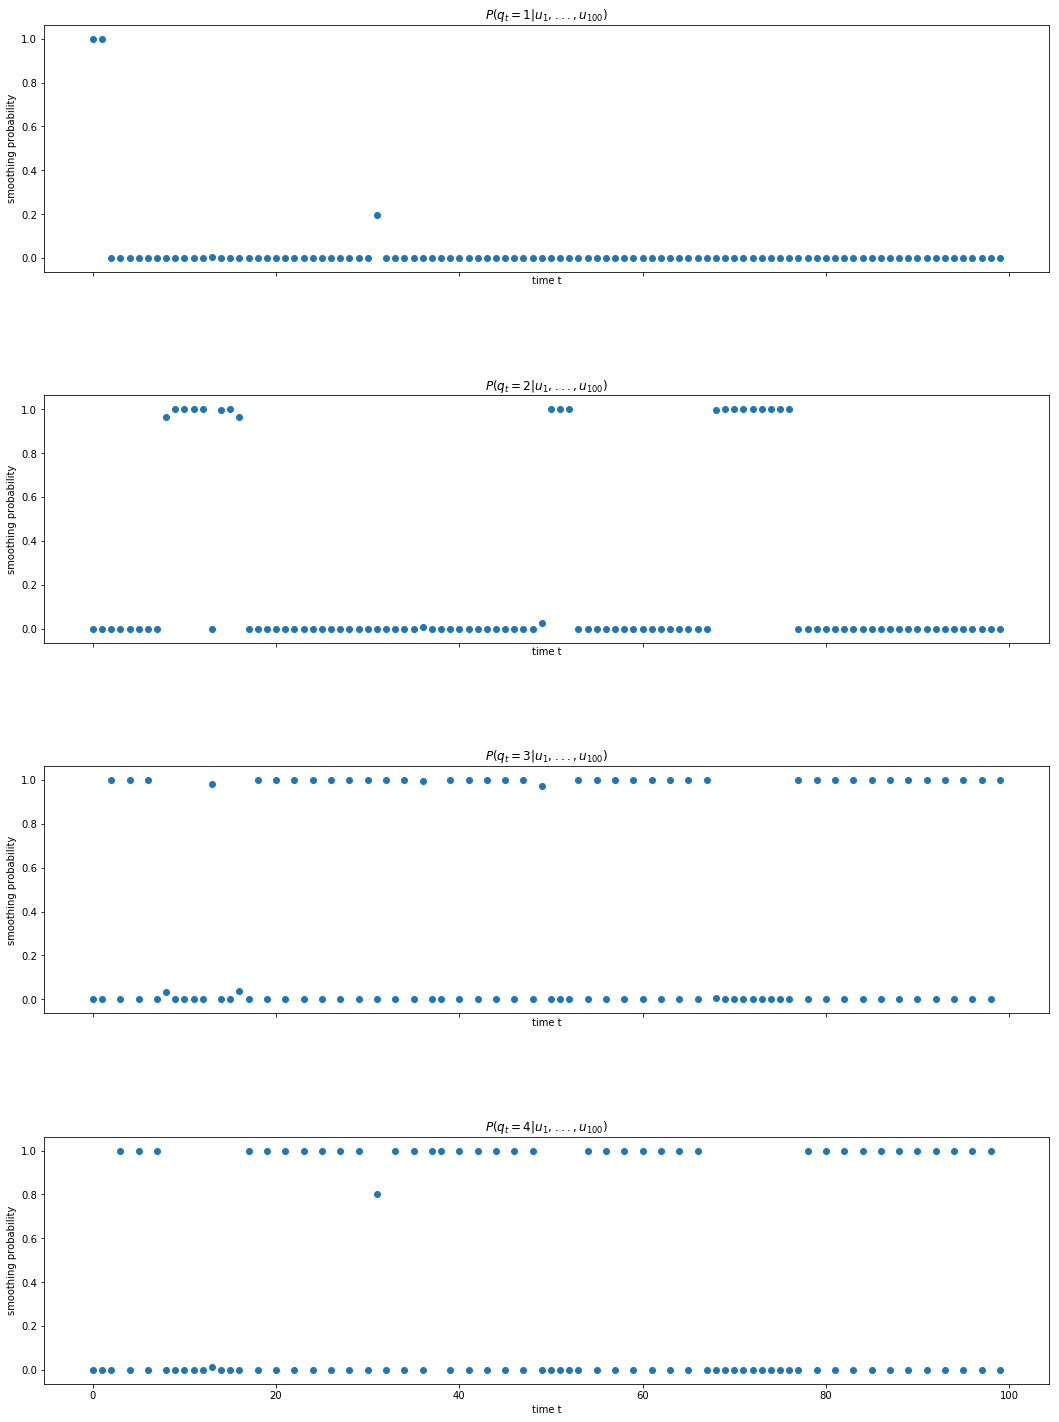
\includegraphics[width=1\linewidth]{images/q9}
\caption{$\mathbb{P}[q_t | u_1, \hdots, u_{T}]$ for $T =100$ for $q_t \in \{1,2,3,4\}$}
\label{fig:prob_test}
\end{figure}

\paragraph{10. Most likely states of the previous points according to theirs marginal probabilities}
The most likely states according to theirs marginal probabilities are shown below

\begin{figure}[H]
\centering
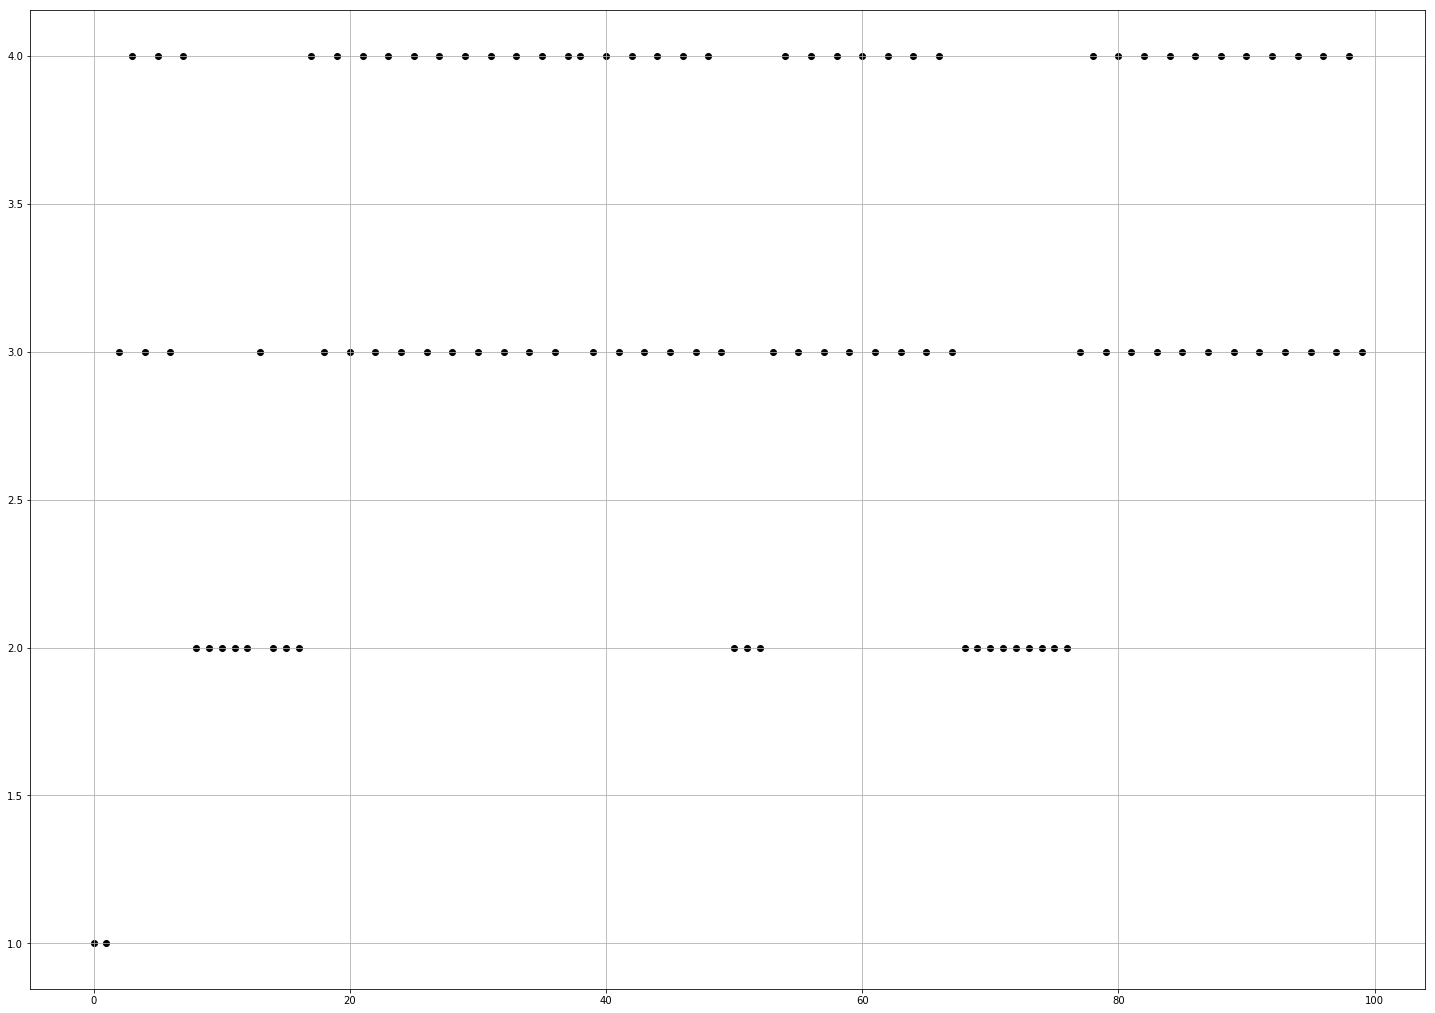
\includegraphics[width=1\linewidth]{images/q10}
\caption{most probable state as a function of time for $\mathbb{P}[q_t | u_1, \hdots, u_{T}]$}
\label{fig:prob_state}
\end{figure}

\paragraph{11. Most likely state of the previous points using Viterbi algorithm}
The most likely state using Viterbi algorithm are shown below:

\begin{figure}[H]
\centering
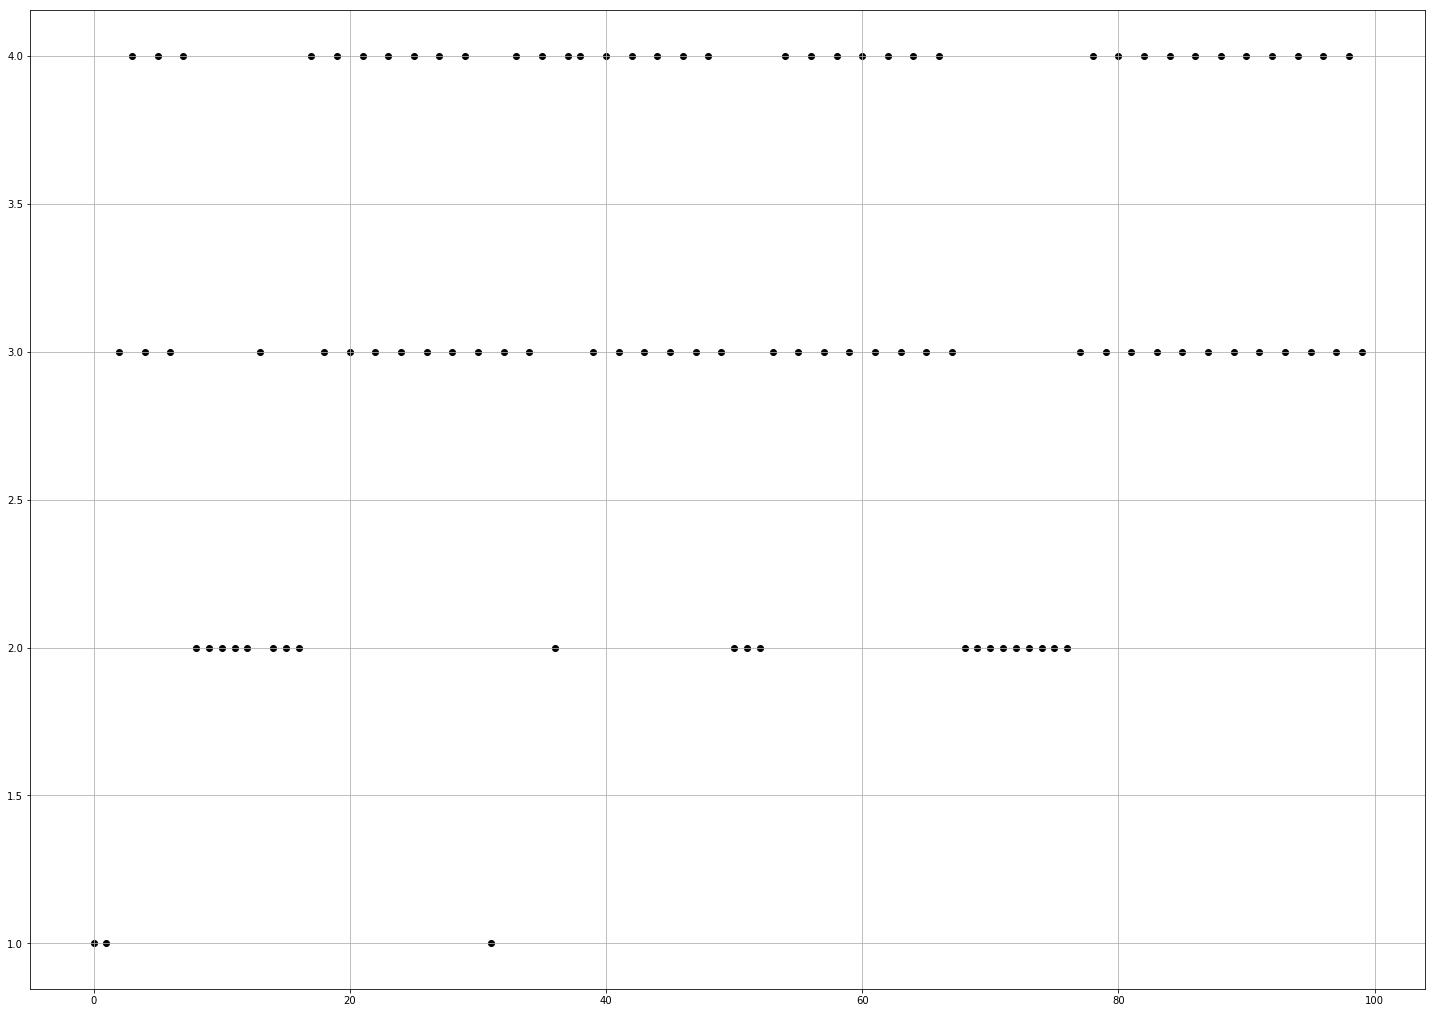
\includegraphics[width=1\linewidth]{images/q11}
\caption{most probable state as a function of time for $\mathbb{P}[q_t | u_1, \hdots, u_{T}]$ using viterbi algorithm}
\label{fig:prob_state_vit}
\end{figure}

As we can see on Figure ~\ref{fig:prob_state_vit}, Viterbi algorithm and the previous question associate almost always the same classes to the data points. Using all the points (500), we can see that the Viterbi algorithm and the previous marginal computation associate the same classes to the data points $97\%$ of the time (485/500) (See code).

\paragraph{12. How would you choose the number of states if you did not know it?}

If the number of states wasn't known I would have chosen $K$ (the number of states) such that it maximizes the log-likelihood obtained by the Expectation Maximization algorithm.

\end{document}
